In this section we will make a quick review of all the models we passed through trying to illustrate its architecture, performance and all the problems we faced in each one and how we adapted to it.
\subsection{CNN Model}
As we mentioned before in the review section, we follow \textbf{Facial Expression Recognition using Convolutional Neural Networks: State of the Art} Paper\cite{state_of_art} model number five,
on \textbf{fer13} dataset, this model follows the paper \textbf{Learning Social Relation Traits from Face Images} with architecture \textbf{CPNCPNCPCFF} \footnote{ the operations C , P ,N ,F denote to covolutional ,Pooling ,Normalization,Fully Connected }, we get accuracy as mentioned in table \ref{tab:14model}
\begin{table}[h!]
	\begin{center}
		\caption{Table of developing Accuracy throw 5 epochs with Batch size 128 and Adadelta optimizer.}
		\label{tab:14model}
		\begin{tabular}{l|c|l|c}
			\textbf{Epoch Number} & \textbf{Training Accuracy} & \textbf{Testing Accuracy} &\textbf{Loss}\\ 
			\hline 
			Epoch 1 & 22.08\% & 13.10\% & 3.6658 \\
			Epoch 2 & 22.23\% & 27.96\% & 3.5919 \\
			Epoch 3 & 23.63\% & 18.54\% & 3.7231 \\
			Epoch 4 & 23.10\% & 27.96\% & 3.4896 \\
			Epoch 5 & 24.42\% & 22.89\% &  3.4968 \\									
			\end{tabular}
	\end{center}

\end{table}
\paragraph{Testing Across Multiple Optimizers}
Over a thousand of both training and testing samples with six epochs we get this final values in table \ref{tab:optimizers}

\paragraph{}
We notice after training this model with more and more epochs that this model fall in \textbf{over-fitting problem}, we found that no matter how many epochs we run the model at certain point the testing accuracy becomes constant and the training accuracy grows more and more without stopping. We notice also that the model is unstable, having unreasonable changes in accuracy. 
\begin{table}[h!]
	\begin{center}
		\caption{Table of developing Accuracy with respect to different Optimizers with learning rate 0.01 \newline}
		\label{tab:optimizers}
		\begin{tabular}{l|c|l}
			\textbf{Optimizer} & \textbf{Training Accuracy} & \textbf{Testing Accuracy}\\ 
			\hline 
			Adadelta & 38.3\% & 36.3\% \\
			Adagrad & 40.2\% & 33\%\\
			Nadam & 36.8\% & 36\% \\
			Adamax & 37.7\% & 32\% \\
		\end{tabular}
	\end{center}
\end{table}
\paragraph{}
Using the FER dataset with Adadelta optimizer, we get a result of 95\% training accuracy and only 33\% testing accuracy.
\subsubsection{Solving Over-Fitting Problem}
\paragraph{} Suggested solutions to solve this problem were:
\begin{enumerate}
	\item Update model layers.
	\item Dealing with dataset problems.
\end{enumerate}
\subsection{Update Model Layers}
\subsubsection{New Structure}
We update our structure as in figure \ref{arch}. 
We use HOG and Landmarks path as feature extraction methods.\newline
Result of this section (without normalization) (mentioned above) is 33\%,
with normalization we get \textbf{testing accuracy of 56.93\%} and \textbf{training accuracy of 74\%} in 10 epochs. 

\begin{figure}
	\centering
	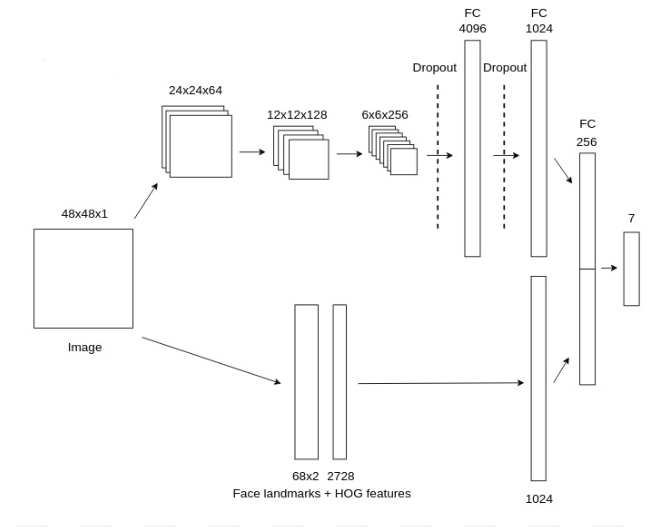
\includegraphics[width=.7\textwidth]{images/Arch.png}
	\caption{model new Architecture}
	\label{arch}
\end{figure}

\subsection{Dealing With Dataset Problems}
One of the datasets we worked on "FER13" was imbalanced, which made the trained model more biased towards negative emotions (which were more presented in the dataset), the solution for this is to balance the data by :
\begin{enumerate}
	\item Under-sampling.
	\item Data Augmentation.
\end{enumerate}
\subsubsection{Under-sampling}
\paragraph{Results}
Unfortunately this made things even worse, since the difference between the sizes of smallest class and other classes was significant (see Figure~\ref{fig:fer13}) so it resulted in a large decrease in data set size which lead to a large decrease in learning.\newline

Table \ref{tab:table1} shows how prediction accuracy of the model changed during training epochs, as the table shows, by more training, the training accuracy increases, while testing accuracy actually decreases, so this technique couldn't help solve the over-fitting problem we had with the previous model which stopped at about 50\% testing accuracy before over-fitting, it even caused a decrease in the accuracy, so this technique wasn't a success in his case. 
\begin{table}[h!]
	\centering
	\caption{This table shows learning progress for model after under-sampling for dataset}
	\label{tab:table1}
	\begin{tabular}{c | c | c | c}
		\textbf{Number of Epochs} & \textbf{Training accuracy} & \textbf{Testing accuracy} & \textbf{Error}\\ \hline 
		10 & 39.33 \% & 37.32 \% & 1.69 \\
		20 & 49.08 \% & 36.80 \% & 1.73 \\
		30 & 53.01 \% & 35.64 \% & 1.83 \\
	\end{tabular}
\end{table}

\subsubsection{Data Augmentation}
Also after applying data-augmentation with horizontal-flip as suggested in the paper\cite{state_of_art}, it made things worse.\newline
figure \ref{tab:table12} after more training we find that testing accuracy stop increasing or sometimes start to decrease .
\begin{table}[h!]
	\centering
	\caption{This table shows learning progress for model after applying data augmentation to the dataset}
	\label{tab:table12}
	\begin{tabular}{c | c | c | c}
		\textbf{Number of Epochs} & \textbf{Training accuracy} & \textbf{Testing accuracy} & \textbf{Error}\\ \hline 
		10 & 15.1\% & 27\% & 1.87 \\
		100 & 20\% &  27\% & 1.5 \\
	\end{tabular}
\end{table}

\subsection{Transfer-learning}
Section \ref{sec:transferlearning} describes what transfer learning is, we choose vgg16 pretrained model to apply.

\paragraph{VGG16}
is a convolutional neural network model built in keras with imageNet dataset, so we apply this method with simple dropout and dense layers and it gave testing accuracy of 27\%.
we found that also vgg16 was not a solution because to use any pretrained model we had to have at least 1000 samples for each class, which we didn't.

\subsection{Auto-Keras}
Auto-keras is a new built-in library in keras, that tries every possible CNN combination in a period chosen by the user to get the best model structure and configuration. It takes training time, training and testing samples as an input, its default training time is 24 hours and we can get the best model and save it from the program.
After running the code, it stuck in the middle and with online searching about this problem, we found that this is a common problem with this library and it seems to be a bug in it or an OS issue.
